\documentclass{beamer}
\usetheme{Madrid}
\newcommand{\z}{\mathbf{z}}
\newcommand{\uout}{u_{out}}
\newcommand{\vout}{v_{out}}
\newcommand{\uoutdum}{u_{out}^{dum}}
\newcommand{\uinplus}{u_{in}^{+}}
\newcommand{\uinminus}{u_{in}^{-}}
\newcommand{\winl}{w_{in}^{l}}
\newcommand{\win}{w_{in}}
\newcommand{\uin}{w_{in}}
\newcommand{\vin}{v_{in}}

\DeclareMathOperator*{\plusrightarrow}{\ensuremath{\xrightarrow{+}}}
\DeclareMathOperator*{\minusrightarrow}{\ensuremath{\xrightarrow{-}}}
\DeclareMathOperator*{\plusleftarrow}{\ensuremath{\xleftarrow{+}}}
\DeclareMathOperator*{\minusleftarrow}{\ensuremath{\xleftarrow{-}}}
\usepackage{multicol, latexsym, amsmath, amssymb}
\usepackage{appendixnumberbeamer} 
\usepackage{xcolor}
\usepackage{algpseudocode}
% \usepackage{algorithm}
% \usepackage{algorithmic}
\usepackage{xr}
\usepackage[linesnumbered,ruled,algo2e]{algorithm2e}

\setbeamertemplate{navigation symbols}{}


\AtBeginSection[]{
  \begin{frame}
  \vfill
  \centering
  \begin{beamercolorbox}[sep=8pt,center,shadow=true,rounded=true]{title}
    \usebeamerfont{title}\insertsectionhead\par%
  \end{beamercolorbox}
  \vfill
  \end{frame}
}

\AtBeginSubsection[]{
  \begin{frame}
  \vfill
  \centering
  \begin{beamercolorbox}[sep=8pt,center,shadow=true,rounded=true]{title}
    \usebeamerfont{title}\insertsubsectionhead\par%
  \end{beamercolorbox}
  \vfill
  \end{frame}
}



\usepackage{subcaption}

\title[DeltaGrad]{Weekly Presentation\\DeltaGrad: Rapid retraining of machine learning models}

\author[Wu et al.~]{Yinjun Wu \and Edgar Dobriban \and Susan B Davidson}
\date{\today}

\begin{document}
\begin{frame}
    \titlepage
\end{frame}

\begin{frame}
    \frametitle{Overview}
    \tableofcontents
\end{frame}


\section{Motivation}
\begin{frame}
    \frametitle{Retaining Problem}
    Regular Pipeline:
    \begin{enumerate}
      \item Train a ML model from data using a learning algorithm
      \item Small change in training data occurs (deletions or additions)
      \item Retrain ML model from scratch
    \end{enumerate}

    \begin{itemize}
      \item<2-> Computationally expensive process
      \item<3-> Throws away useful computations from initial training
    \end{itemize}
    \begin{block}<4->{Research Question}
      Can we retrain models in an efficient manner?
    \end{block}
\end{frame}

\begin{frame}
  \frametitle{Potential Applications}
  \begin{itemize}
    \item<1-> \textbf{GDPR}: Deletion of private information from public datasets
    \item<2-> \textbf{Continuous Model Updating}: Handle additions, deletions and changes of training samples
    \item<3-> \textbf{Data Valuation}: \textit{Leave One Out} tests to find important training samples 
    \item<4-> \textbf{Bias Reduction}: Speeds up jackknife resampling that requires retrained model parameters 
  \end{itemize}
  

\end{frame}
\section{Related Work}

\begin{frame}
  \frametitle{Prior Work}
  \begin{itemize}
    \item Prior work for specialized problems and ML models, usually for deletion
    \begin{itemize}
      \item Provenane Based deletions for linear and logistic regression \cite{wuPrIUProvenanceBasedApproach2020}
      \item Newton step and noise for \textit{certified data removal} \cite{guoCertifiedDataRemoval2020}
      \item K-means clustering \cite{ginartMakingAIForget2019}
    \end{itemize}
  \end{itemize}
\end{frame}

\section{DeltaGrad}
\begin{frame}
  \frametitle{Gradient Descent}
  \begin{itemize}
    \item Objective function  
    \[
        F(\w) = \frac{1}{n}\sum_{i=1}^{n}F_{i}(\w)  
    \]
    \item Stochastic Gradient Descent update rule, $\mathcal{B}_{t}$ is randomly sampled mini-batch of size $B$
    \[
      \w_{t+1} \leftarrow \w_{t}-\frac{\eta_{t}}{B} \sum_{i \in \mathcal{B}_{t}} \nabla F_{i}\left(\w_{t}\right) 
    \]
    \item Full-batch gradient descent (GD) is on entire data 
    \[
      \w_{t+1} \leftarrow \w_{t}-\frac{\eta_{t}}{n} \sum_{i=1}^{n} \nabla F_{i}\left(\w_{t}\right) 
    \]
  \end{itemize} 
\end{frame}

\begin{frame}
  \frametitle{Removal of data}
  \begin{itemize}
    \item After training,  $R = \{i_1,i_2,\dots,i_r\}$ is removed, where $r \ll n$
    \item Naive retraining is applying GD over remaining samples, $\w^{U}$ is resulting parameters
    \begin{align}\label{eq: update_rule_naive} 
      & \uw_{t+1} \leftarrow \uw_{t} - \frac{\eta_t}{n-r}\sum_{\substack{i \not\in R}} \nabla F_i\left(\uw_{t}\right) 
    \end{align}
    \item The explicit gradient computation $\sum_{\substack{i \not\in R}} \nabla F_i\left(\uw_{t}\right)$ is expensive
    \item Instead rewrite \eqref{eq: update_rule_naive} as follows 
    \begin{align}\label{eq: approx_w_t}
      \begin{split}
      \uw_{t+1} 
               = \uw_{t} - \frac{\eta_t}{n-r}\left[\sum_{i=1}^{n} \nabla F_{i}\left(\uw_{t}\right) - \sum_{\substack{i \in R}} \nabla F_i\left(\uw_{t}\right)\right].
      \end{split}
      \end{align}
      \item $\sum_{\substack{i \in R}} \nabla F_i\left(\uw_{t}\right)$ is cheaper to compute
  \end{itemize}
\end{frame}

\begin{frame}
  \frametitle{Etymology}
  \begin{itemize}
    \item After a small change to the data we need to redo the SGD computations
    \item We can achieve this by understanding the \textit{delta} of the Gradient Descent 
    \[ 
      n\nabla F(\w) = \sum_{i=1}^{n}\nabla F_{i}(\w_t) \quad \& \quad n\nabla F(\uw) =  \sum_{i=1}^{n} \nabla F_{i}\left(\uw_{t}\right)
    \]
    \item Hence, the approach is called \textit{DeltaGrad}
  \end{itemize}
\end{frame}

\begin{frame}
  \frametitle{Aprroximating $\nabla F(\uw)$}
  \begin{itemize}
    \item $\w_{0}$, $\dots,\w_{t}$ and $\nabla F\left(\w_{0}\right)$, $\dots, \nabla F\left(\w_{t}\right)$ are cached from training on initial dataset
    \item By Cauchy mean-value theorem\footnote<2->{Seems to be a consequence of Fundamental theory of Calculus and mean-value theorem}
    \[
      \nabla F(\uw_{t}) - \nabla F(\w_{t}) = \bH_{t} \cdot (\uw_{t} - \w_{t}) 
    \]
    Where $\bH_{t} = \int_{0}^{1}\bH(\w_{t}+x(\uw_{t}-\w_{t}))dx$ is the integrated hessian
    \item This requires a hessian $\bH_{t}$ at each step, which is expensive to maintain and evaluate
    \item Leverage classical L-BFGS algorithm to approximate $\bH_{t}$
  \end{itemize}
\end{frame}

\begin{frame}
  \frametitle{Review of L-BFGS}
  \begin{itemize}
    \item Traditional L-BFGS updates gradients using
    \[\nabla F(\w_{t+1}) - \nabla F(\w_{t})  = \B_{t} \cdot (\w_{t+1}-\w_{t}) \]
    Where, $\B_t$ is the approximation of the hessian
  \end{itemize}
  \vfill
  \scalebox{0.8}{\begin{minipage}{0.55\textwidth}
    Traditional L-BFGS
          \[
  \begin{array}{l}
  \nabla F\left(\w_{t+1}\right)-\nabla F\left(\w_{t}\right) \approx \mathbf{B}_{t}\left(\w_{t+1}-\w_{t}\right) \\
  \mathbf{B}_{t} \approx \mathbf{H}_{t} \\
  =\int_{0}^{1} \mathbf{H}\left(\w_{t}+x\left(\w_{t+1}-\w_{t}\right)\right) d x \\
  \s_{t}=\w_{t+1}-\w_{t} \\
  \y_{t}=\nabla F\left(\w_{t+1}\right)-\nabla F\left(\w_{t}\right)
  \end{array}
    \]
  \end{minipage}}
  \hfill%
  \scalebox{0.8}{
  \begin{minipage}{0.55\textwidth}
    L-BFGS for approximating $\nabla F(\uw)$
          \[
  \begin{array}{l}
  \nabla F\left(\uw_{t}\right)-\nabla F\left(\w_{t}\right) \approx \mathbf{B}_{t}\left(\uw_{t}-\w_{t}\right) \\
  \mathbf{B}_{t} \approx \mathbf{H}_{t} \\
  =\int_{0}^{1} \mathbf{H}\left(\w_{t}+x\left(\uw_{t}-\w_{t}\right)\right) d x \\
  \s_{t}=\uw_{t}-\w_{t} \\
  \y_{t}=\nabla F\left(\uw_{t}\right)-\nabla F\left(\w_{t}\right)
\end{array}
  \]
    \end{minipage}}
\end{frame}

\begin{frame}
  \frametitle{Using L-BFGS}
  \begin{itemize}
    \item Maintain $m$ historical observations of $\textbf{Y} = (\y_{t},\y_{t-1},\dots,\y_{t-m})$ and $\textbf{S} = (\s_{t},\s_{t-1},\dots,\s_{t-m})$
    \item Let $g$ be a function defined by L-BFGS, then we can approximate $\B_{t}\cdot\textbf{v}$ using 
    \[
        g(\textbf{Y},\textbf{S},\textbf{v}) 
    \]
    Where, $\textbf{v}$ is an arbitrary vector.
    \item Therefore,  
    \[ \B_{t}\cdot(\uw_{t}-\w_{t}) = g(\textbf{Y},\textbf{S},\uw_{t}-\w_{t}) \]
    \item Hence we obtain the approximation as 
    \[
        \nabla F(\uw_{t}) \approx \nabla F(\w_{t}) + \B_{t} \cdot (\uw_{t}-\w_{t}) 
    \]
  \end{itemize}
\end{frame}

\begin{frame}
  \frametitle{Rewriting}
  \begin{itemize}
    \item Denoting $\iw$ as the approximate $\uw$ we have 
    \[
      \nabla F(\iw_{t}) \approx \nabla F(\w_{t}) + \B_{t} \cdot (\iw_{t}-\w_{t}).
    \]
    \item replacing in \eqref{eq: approx_w_t}
    \[\iw_{t+1}  = \iw_{t} - \frac{\eta_{t}}{n-r} \left\{ n[\B_{t}(\iw_t - \w_t) + \nabla F(\w_t)] - \sum_{i\in R} \nabla F(\iw_t)\right\}\]
  \end{itemize}
\end{frame}


\begin{frame}
  \frametitle{Problem with Error Bound}
  \includegraphics[page=43,clip,trim=0.5cm 1cm 0cm 1cm,width=\textwidth]{images/Slides.pdf}
\end{frame}

\begin{frame}
  \frametitle{Controlling the Errors}
  \begin{itemize}
    \item Do explicit evaluations for $j_{0}$ "burn-in" iterations and then periodically every $T_{0}$ iterations
    \includegraphics[page=46,clip,trim=0.5cm 1cm 0cm 1cm,width=0.9\textwidth]{images/Slides.pdf}
  \end{itemize}
\end{frame}

\begin{frame}
  \frametitle{Benefit of DeltaGrad}
  \begin{itemize}
    \item DeltaGrad can be extended to when $r$ samples are added rather than deleted
    \item Change the $+$ to minus in the update formula to get 
    \[
      \iw_{t+1}  = \iw_{t} - \frac{\eta_{t}}{n\textcolor{red}{+}r} \left\{ n[\B_{t}(\iw_t - \w_t) + \nabla F(\w_t)] \textcolor{red}{+} \sum_{i\in R} \nabla F(\iw_t)\right\}
    \]
    \item Here $\sum_{i\in R} \nabla F(\iw_t)$ is the gradient of the added $r$ samples
  \end{itemize}
  
\end{frame}

\begin{frame}[fragile]
  \frametitle{Algorithm}
  % 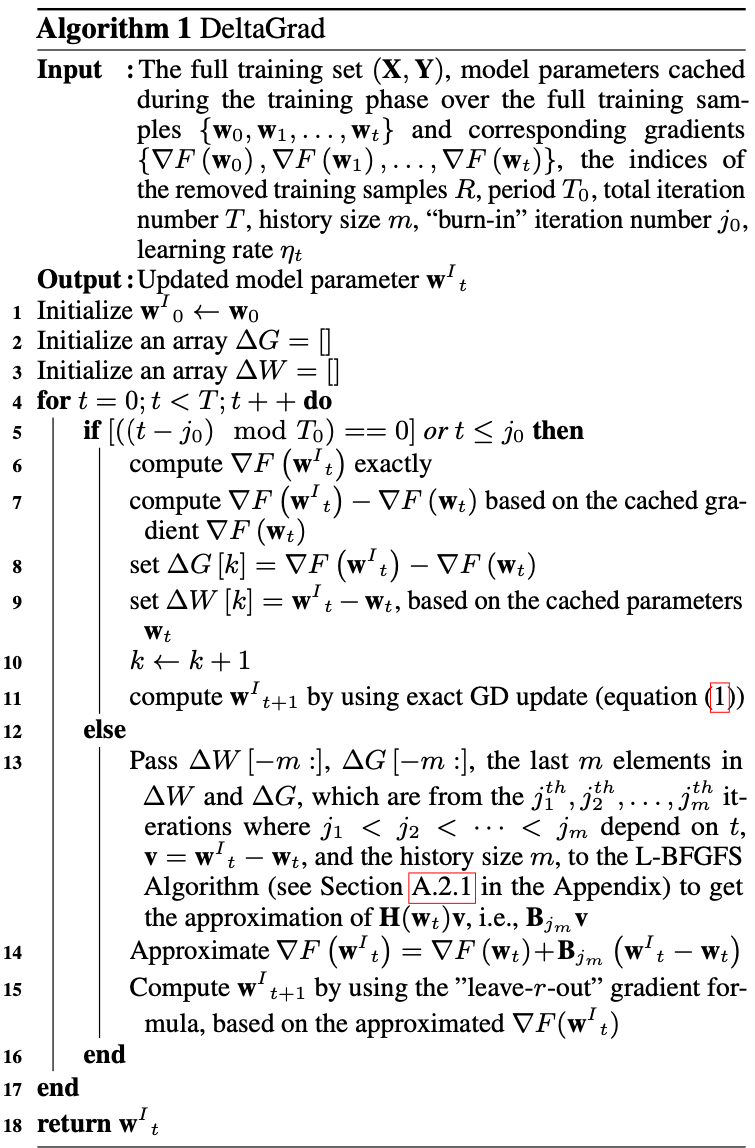
\includegraphics[width=0.4\textwidth]{images/Screenshot 2020-09-29 at 17.10.21.png}
  
\begin{algorithm}[H] 
  \small
  % \footnotesize
  % \SetKwInOut{Input}{Input}
  % \SetKwInOut{Output}{Output}
  % \Input{The full training set $\left(\textbf{X}, \textbf{Y}\right)$, model parameters cached during the training phase over the full training samples $\{\w_{0}, \w_{1}, \dots, \w_{t}\}$ and corresponding gradients $\{\nabla F\left(\w_{0}\right), \nabla F\left(\w_{1}\right), \dots, \nabla F\left(\w_{t}\right)\}$, the indices of the removed training samples $R$, period $T_0$, total iteration number $T$, history size $m$, ``burn-in'' iteration number $j_0$, learning rate $\eta_t$}
  % \Output{Updated model parameter $\iw_{t}$}
  % Initialize $\iw_{0} \leftarrow \w_{0}$
  
  % Initialize an array $\Delta G = \left[\right]$
  
  % Initialize an array $\Delta W = \left[\right]$
  
  % \For{$t=0;t<T; t++$}{
  
  % \eIf{$[((t-j_0) \mod T_0) == 0]$ or $t \leq j_0$}
  % {
  %     compute $\nabla F\left(\iw_{t}\right)$ exactly
      
  %     compute $\nabla F\left(\iw_{t}\right) - \nabla F\left(\w_{t}\right)$ based on the cached gradient $\nabla F\left(\w_{t}\right)$
      
  %     set $\Delta G\left[k\right] = \nabla F\left(\iw_{t}\right) - \nabla F\left(\w_{t}\right)$
      
  %     set $\Delta W\left[k\right] = \iw_{t} - \w_{t}$, based on the cached parameters $\w_{t}$
      
  %     $k\leftarrow k+1$
      
  %     compute $\iw_{t+1}$ by using exact GD update (equation \eqref{eq: update_rule_naive})
  % }
  % {
  %     Pass $\Delta W\left[-m:\right]$, $\Delta G\left[-m:\right]$, the last $m$ elements in $\Delta W$ and $\Delta G$, which are from the $j_1^{th}, j_2^{th},\dots, j_m^{th}$ iterations where $j_1 < j_2< \dots < j_m$ depend on $t$, $\textbf{v} = \iw_{t} - \w_{t}$, and the history size $m$, to the L-BFGFS Algorithm (see Section \ref{sec: quasi_newton} in the Appendix) to get the approximation of $\bH(\w_{t})\textbf{v}$, i.e., $\B_{j_m}\textbf{v}$
      
  %     Approximate $\nabla F\left(\iw_{t}\right) = \nabla F\left(\w_{t}\right) + \B_{j_m}\left(\iw_{t} - \w_{t}\right)$
      
  %     Compute $\iw_{t+1}$ by using the "leave-$r$-out" gradient formula, based on the approximated $\nabla F(\iw_{t})$ 
  % }
  % }
  
  \Return $\iw_{t}$
  \caption{DeltaGrad}
  \label{alg: update_algorithm}
  \end{algorithm}

\end{frame}
\section{Theoretical Results}

\section{Experimental Results}

\bibliography{UpdateMl}
\bibliographystyle{alpha}

\appendix
\section{Large Deletions}
\begin{frame}
  \frametitle{Large Deletions}


\end{frame}



\end{document}  